\section{Two-magnon continua and magnon--phonon modes}\label{sec:14.2}

In NiO, linear spin-wave theory assigns to the component of each nickel spin along the ordered moment a fluctuation weight equal to \SI{7}{\percent} of the one-magnon weight (\cref{we:14-nio}), carried entirely by magnon pairs, which that component creates (\cref{sec:7.1}). Each pair shares the momentum transfer between its two members, so at a small momentum transfer the pair can take up any energy from the one-magnon energy to twice the top of the magnon band, \SI{236}{meV}. The pairs thus decouple the energy deposited from the momentum transfer, which matters for the lightest dark matter. In the effective theory of gapless antiferromagnetic magnons, the two-magnon channel extends the projected reach of NiO, MnO and Cr$_2$O$_3$ down to masses of about \SI{1}{keV}~\cite{esposito2023optimal}. The lattice adds a second correction. Through spin--orbit coupling a strain changes the magnetic anisotropy energy, and a magnon and a phonon of the same wavevector and energy mix into hybrid modes. Together with the one-magnon weight defect of \cref{sec:14.1}, the pairs, their final-state interaction and the hybrids are the corrections in $1/|\vect{S}|$ and in the magnetoelastic coupling to the one-magnon rate, and for NiO we size each.

\subsection{Two-magnon amplitude and response}\label{sec:14.2-amp}

Take the two-sublattice antiferromagnet of \cref{sec:7.1}, with the moments along $\pm\hat{\vect{z}}$, and the longitudinal ionic spin at wavevector $\vect{q}$, $S^z(\vect{q}) = \sum_j\ee^{\ii\vect{q}\cdot\vect{r}_j}S^z_j$. On sublattice A, $S^z_i = |\vect{S}| - d^\dagger_{\mathrm{A}i}d_{\mathrm{A}i}$, and on B, $S^z_j = -|\vect{S}| + d^\dagger_{\mathrm{B}j}d_{\mathrm{B}j}$, exactly, by \cref{eq:7.1-HP}. The constants give the magnetic Bragg peaks, at $\omega = 0$, and deposit no energy. The rest is bilinear in the bosons. With the Fourier convention of \cref{sec:7.1} on each sublattice, the lattice sums give
\begin{equation*}
  S^z(\vect{q}) = -\sum_{\vect{k}}d^\dagger_{\mathrm{A}\vect{k}}\,d_{\mathrm{A},\vect{k}-\vect{q}} + \sum_{\vect{k}}d^\dagger_{\mathrm{B}\vect{k}}\,d_{\mathrm{B},\vect{k}+\vect{q}} + (\text{Bragg}) ,
\end{equation*}
with $\vect{k}$ over the $N_{\mathrm{s}}$ wavevectors of the zone of one sublattice. Now insert the inverse Bogoliubov transformation \cref{eq:D.19-inverse}, $d_{\mathrm{A}\vect{k}} = u^{\mathrm{M}}_{\vect{k}}a_{\vect{k}1} - v^{\mathrm{M}}_{\vect{k}}a^\dagger_{\vect{k}2}$ and $d_{\mathrm{B}\vect{k}} = u^{\mathrm{M}}_{\vect{k}}a_{\vect{k}2} - v^{\mathrm{M}}_{\vect{k}}a^\dagger_{\vect{k}1}$. At $T = 0$ only the terms with two creation operators survive acting on the magnon vacuum $|0\rangle$. The A term contributes $u^{\mathrm{M}}_{\vect{k}}v^{\mathrm{M}}_{\vect{k}-\vect{q}}\,a^\dagger_{\vect{k}1}a^\dagger_{\vect{k}-\vect{q},2}$, and the B term, after the relabeling $\vect{k} + \vect{q} \to \vect{k}$, contributes $-v^{\mathrm{M}}_{\vect{k}}u^{\mathrm{M}}_{\vect{k}-\vect{q}}$ times the same pair. Hence
\begin{equation}
  S^z(\vect{q})|0\rangle = \sum_{\vect{k}}\mathcal{A}^{\mathrm{2m}}_{\vect{k}}(\vect{q})\,a^\dagger_{\vect{k}1}a^\dagger_{\vect{k}-\vect{q},2}|0\rangle , \qquad
  \mathcal{A}^{\mathrm{2m}}_{\vect{k}}(\vect{q}) = u^{\mathrm{M}}_{\vect{k}}v^{\mathrm{M}}_{\vect{k}-\vect{q}} - v^{\mathrm{M}}_{\vect{k}}u^{\mathrm{M}}_{\vect{k}-\vect{q}} ,
  \label{eq:14.2-amp}
\end{equation}
apart from the Bragg term. The first magnon carries the crystal momentum $\vect{k}$ and lowers the total $S^z$ by one; the second carries $\vect{q} - \vect{k}$, since $a_{\vect{k}2}$ destroys $-\vect{k}$ in the convention of \cref{sec:7.1}, and raises $S^z$ by one. The pair has the momentum $\vect{q}$ and no net spin, as a longitudinal operator requires. The wavevector $\vect{k} - \vect{q}$ may leave the zone of one sublattice. We then compute $u^{\mathrm{M}}$ and $v^{\mathrm{M}}$ at that wavevector from $A_{\vect{k}}$ and $B_{\vect{k}} = J^{\mathrm{ex}}_{\mathrm{AB}}(\vect{k})$ with its sign. Since $J^{\mathrm{ex}}_{\mathrm{AB}}$ changes by at most a sign under a reciprocal vector of the sublattice, $v^{\mathrm{M}}$ does too, and $|\mathcal{A}^{\mathrm{2m}}_{\vect{k}}|^2$ does not depend on which representative is used.

A ferromagnet has $v^{\mathrm{M}} \equiv 0$ and no amplitude, and at $T = 0$ no inelastic longitudinal response at all, beyond linear order as well (\cref{sec:14.1}). In an antiferromagnet the amplitude vanishes at $\vect{q} = 0$, where $u_{\vect{k}}v_{\vect{k}} - v_{\vect{k}}u_{\vect{k}} = 0$, and at every reciprocal vector of the lattice of magnetic ions, where $S^z(\vect{q})$ is the total $S^z$, which commutes with $H_{\mathrm{H}}$ and creates nothing. For small $\vect{q}$, with $u^{\mathrm{M}} = \cosh\theta_{\vect{k}}$ and $v^{\mathrm{M}} = \sinh\theta_{\vect{k}}$, the amplitude is $\mathcal{A}^{\mathrm{2m}}_{\vect{k}} = \sinh(\theta_{\vect{k}-\vect{q}} - \theta_{\vect{k}}) \simeq -\vect{q}\cdot\nabla_{\vect{k}}\theta_{\vect{k}}$, and the weight grows as $q^2$. Near the ordering wavevector $v^{\mathrm{M}}_{\vect{k}-\vect{q}}$ has the opposite sign to $v^{\mathrm{M}}_{\vect{k}}$, the two terms add, and the amplitude approaches $2u^{\mathrm{M}}_{\vect{k}}v^{\mathrm{M}}_{\vect{k}} = \sinh2\theta_{\vect{k}}$, its largest value. Physically, $S^z(\vect{q})$ near the ordering wavevector measures the fluctuation of the staggered moment, which the zero-point motion of the spin waves makes large.

The response follows as in \cref{sec:7.1}. The electron spin density along the moments is $s_{e,z}(\vect{q}) = F^{\mathrm{mag}}(q)S^z(\vect{q})$ by \cref{eq:7.1-Fmag}. The pair states of \cref{eq:14.2-amp} are orthonormal, and each appears once in the sum over $\vect{k}$. With $N = 2N_{\mathrm{s}}$ magnetic ions, $\Omega_{\mathrm{ion}}$ the volume per ion and $\Vol = N\Omega_{\mathrm{ion}}$, \cref{eq:4.2-Sab} gives:
\begin{keyresult}[Two-magnon spin response of a collinear antiferromagnet]
\begin{equation}
  S^{(2\mathrm{m})}_{zz}(\vect{q},\omega) = \frac{2\pi}{\Omega_{\mathrm{ion}}}\,|F^{\mathrm{mag}}(q)|^2\,\frac{1}{2N_{\mathrm{s}}}\sum_{\vect{k}}\bigl|\mathcal{A}^{\mathrm{2m}}_{\vect{k}}(\vect{q})\bigr|^2\,\delta\bigl(\omega - \omega^{\mathrm{M}}_{\vect{k}} - \omega^{\mathrm{M}}_{\vect{k}-\vect{q}}\bigr) ,
  \label{eq:14.2-S2m}
\end{equation}
for $T = 0$ and $\omega > 0$, with $z$ along the moments and $\mathcal{A}^{\mathrm{2m}}$ of \cref{eq:14.2-amp}. Its weight and that of the one-magnon line at the same $\vect{q}$ are in the ratio $w_\parallel(\vect{q})/w_\perp(\vect{q})$ of the weights per ion
\begin{equation}
  w_\parallel(\vect{q}) = \frac{1}{2N_{\mathrm{s}}}\sum_{\vect{k}}\bigl|\mathcal{A}^{\mathrm{2m}}_{\vect{k}}(\vect{q})\bigr|^2 , \qquad
  w_\perp(\vect{q}) = |\vect{S}|\,w^{\mathrm{M}}_{\vect{q}} ,
  \label{eq:14.2-wpar}
\end{equation}
with $w^{\mathrm{M}}_{\vect{q}}$ the one-magnon weight of \cref{eq:14.1-Safm}.
\end{keyresult}
\noindent Here $w_\perp$ is the $\omega$-integral of $S_{xx} + S_{yy}$ in units of $(2\pi/\Omega_{\mathrm{ion}})|F^{\mathrm{mag}}|^2$. The one-magnon weight is of order $|\vect{S}|$ and the two-magnon weight of order $|\vect{S}|^0$, since the Bogoliubov coefficients do not depend on $|\vect{S}|$: the pairs are a correction of relative order $1/|\vect{S}|$. \Cref{eq:14.2-S2m} is the longitudinal structure factor that Huberman and collaborators compared with the two-magnon continuum of the square-lattice antiferromagnet Rb$_2$MnF$_4$ measured by neutron scattering~\cite[Eq.~(5)]{huberman2005two}. A dark-matter model enters through $\mathfrak{D}_{zz}S^{(2\mathrm{m})}_{zz}$ in \cref{eq:8.2-spectrum}, in the frame of the moments. For a coupling isotropic in the electron spin, $\mathfrak{D}_{ab} \propto \delta_{ab}$, the two-magnon and one-magnon parts of $\sum_a\mathfrak{D}_{aa}S_{aa}$ at fixed $\vect{q}$ are in the ratio $w_\parallel/w_\perp$, whatever the direction of the moments in each domain.

Averaged over $\vect{q}$, $v^{\mathrm{M}}_{\vect{k}-\vect{q}}$ takes both signs equally often, the cross term of $|\mathcal{A}^{\mathrm{2m}}|^2$ drops out, and with $\langle(u^{\mathrm{M}})^2\rangle = 1 + \Delta S$ and $\langle(v^{\mathrm{M}})^2\rangle = \Delta S$, where $\Delta S$ is the zero-point spin reduction of \cref{sec:14.1}, the average of $w_\parallel$ is $\frac12\cdot2(1 + \Delta S)\Delta S = W_\parallel$, while the average of $w_\perp$ is $|\vect{S}|(1 + 2\Delta S) = W_\perp$. \Cref{eq:14.2-wpar} thus resolves the ratio $W_\parallel/W_\perp$ of \cref{sec:14.1} in momentum transfer, which is what a rate needs, since light dark matter samples only small $q$.

\Cref{fig:14-weights} shows the two weights of NiO in linear spin-wave theory with the exchange constants of \cref{eq:7.1-NiO}. At small $q$ along $[111]$ the one-magnon weight rises as $w_\perp \simeq 0.29\,qa$, and the two-magnon weight as $w_\parallel \simeq 0.015\,(qa)^2$, so the ratio vanishes linearly. At $\vect{q} = (\frac14,\frac14,\frac14)2\pi/a$, a momentum transfer of \SI{1.29}{keV}, $w_\perp = 1.00$ and $w_\parallel = 0.081$; along $[111]$ the ratio $w_\parallel/w_\perp$ peaks at 0.082 near \SI{1.4}{keV} and stays below 0.05 under \SI{0.5}{keV}. Toward the ordering wavevector $w_\perp$ diverges while $w_\parallel$ stays finite, near 0.25, and the ratio falls again, averaging over the zone to the $W_\parallel/W_\perp$ of \cref{we:14-nio}.

\begin{figure}[tbp]
  \centering
  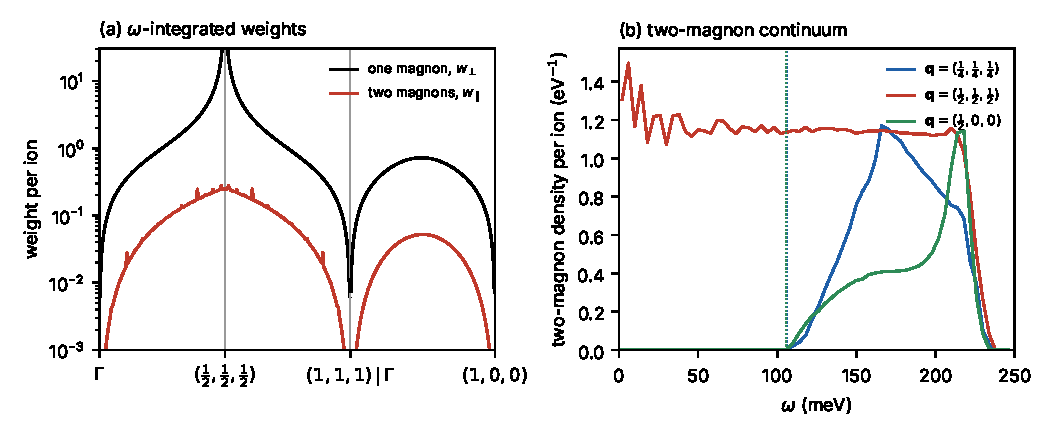
\includegraphics[width=\linewidth]{figures/ch14/fig14_2.pdf}
  \caption{One- and two-magnon weights of NiO in linear spin-wave theory: Heisenberg model with $J_1 = \SI{-1.37}{meV}$ and $J_2 = \SI{19.01}{meV}$ (antiferromagnetic $J^{\mathrm{ex}} > 0$, pairs counted once), $|\vect{S}| = 1$, type-II order on the undistorted fcc lattice, no anisotropy, $T = 0$, magnetic form factor set to one. (a) Weights per ion, integrated over energy, of the transverse one-magnon response, $w_\perp$ (both branches), and of the longitudinal two-magnon response, $w_\parallel$. The path runs along $[111]$ from $\Gamma$ through the ordering wavevector $(\frac12,\frac12,\frac12)$ to $(1,1,1)$, which is equivalent to $\Gamma$, and from $\Gamma$ to $(1,0,0)$; wavevectors in units of $2\pi/a$, $a = \SI{4.17}{\angstrom}$. Both vanish at $\Gamma$ and $(1,1,1)$, where the total longitudinal spin is conserved; $w_\perp$ diverges at the ordering wavevector and vanishes at $(1,0,0)$, a soft point of the undistorted model, where $w_\parallel$ is small and would vanish for $J_1 = 0$. (b) Two-magnon density per ion, $(\Omega_{\mathrm{ion}}/2\pi)S^{(2\mathrm{m})}_{zz}/|F^{\mathrm{mag}}|^2$, against energy at three wavevectors (4-meV bins, $3\times10^6$ sampled wavevectors). The dotted lines mark the one-magnon energy at the same wavevector, zero at the ordering wavevector.}
  \label{fig:14-weights}
\end{figure}

\subsection{Kinematic boundaries of the continuum}\label{sec:14.2-edges}

At fixed $\vect{q}$, \cref{eq:14.2-S2m} has weight only between the lower edge $\omega_-(\vect{q}) = \min_{\vect{k}}(\omega^{\mathrm{M}}_{\vect{k}} + \omega^{\mathrm{M}}_{\vect{k}-\vect{q}})$ and the upper edge $\omega_+(\vect{q}) = \max_{\vect{k}}(\omega^{\mathrm{M}}_{\vect{k}} + \omega^{\mathrm{M}}_{\vect{k}-\vect{q}}) \le 2\max_{\vect{k}}\omega^{\mathrm{M}}_{\vect{k}}$. Putting one magnon at a zero of the dispersion, $\vect{k} = 0$, shows that $\omega_- \le \omega^{\mathrm{M}}_{\vect{q}}$; for a dispersion that rises linearly and then bends over, as in NiO, $\omega^{\mathrm{M}}_{\vect{k}} + \omega^{\mathrm{M}}_{\vect{k}-\vect{q}} \ge \omega^{\mathrm{M}}_{\vect{q}}$, and the lower edge is the one-magnon branch itself. The weight at the lower edge is small, because $|\mathcal{A}^{\mathrm{2m}}|^2$ diverges only as $1/k$ near $\vect{k} = 0$ while the phase space closes as $k^2$. In NiO the continuum at $(\frac14,\frac14,\frac14)2\pi/a$ runs from the one-magnon energy, \SI{105.8}{meV}, to \SI{236}{meV}, and at the ordering wavevector it runs from zero, where both magnons sit at zeros of the dispersion, to \SI{236}{meV} (\cref{fig:14-weights}b). The anisotropy that \cref{eq:7.1-heis} leaves out gaps the magnons by less than \SI{5}{meV} in NiO; a gap $\omega_{\mathrm{gap}}$ in both branches moves the lower edge to at least $2\omega_{\mathrm{gap}}$ and leaves the rest of the continuum in place. At $T > 0$ the operator $S^z$ also scatters a thermal magnon into another, with weight proportional to the occupation, which vanishes for temperatures far below the gap.

The continuum changes what dark matter can deposit. Energy conservation, \cref{eq:1.3-omegaq}, allows $\omega \le qv - q^2/2\mchi$, and the one-magnon channel opens at \cref{eq:14.1-mmin}. A pair, however, can take any energy in its continuum, which at small $q$ reaches far above $c_{\mathrm{M}}q$, so the only limit is \cref{eq:1.3-omegamax}, $\omega \le \frac12\mchi v^2$, reached at $q = \mchi v$. For a threshold $E_{\mathrm{th}}$ the two-magnon channel opens at the threshold mass \cref{eq:1.3-mmin}, $2E_{\mathrm{th}}/v_{\mathrm{max}}^2$. The one-magnon channel opens at $E_{\mathrm{th}}/[2c_{\mathrm{M}}(v_{\mathrm{max}} - c_{\mathrm{M}})]$, larger by the factor
\begin{equation}
  \frac{v_{\mathrm{max}}^2}{4c_{\mathrm{M}}(v_{\mathrm{max}} - c_{\mathrm{M}})} \simeq \frac{v_{\mathrm{max}}}{4c_{\mathrm{M}}} \qquad (c_{\mathrm{M}} \ll v_{\mathrm{max}}) .
  \label{eq:14.2-mratio}
\end{equation}
For NiO, with the fastest magnon speed of the $J_1$--$J_2$ model, $c_{\mathrm{M}} = 1.36\times10^{-4}$ (\cref{sec:14.1}), the factor is 5.1: at $E_{\mathrm{th}} = \SI{1}{meV}$ one magnon needs $\mchi \ge \SI{1.46}{keV}$ and two magnons $\mchi \ge \SI{0.285}{keV}$. NiO gains little because its magnons are fast, $c_{\mathrm{M}} \approx v_{\mathrm{max}}/19$; a magnet with slower magnons gains in proportion to $v_{\mathrm{max}}/c_{\mathrm{M}}$. Near the two-magnon edge, however, the momentum transfer $q = \mchi v_{\mathrm{max}}$ is below an eV, $(qa)^2 \sim 10^{-6}$, and the $q^2$ law of $w_\parallel$ makes the rate tiny there; the linear law of $w_\perp$ suppresses the one-magnon rate near its own edge less. The reach in mass thus lies well above the kinematic edge, more so for the pair.

\subsection{Final-state interactions and bound pairs}\label{sec:14.2-fsi}

The two magnons of \cref{eq:14.2-amp} do not move independently. Linear spin-wave theory dropped the terms of fourth order in the bosons, and they act between the members of the pair. For an antiparallel bond the longitudinal part $S^z_iS^z_j = (|\vect{S}| - n_{\mathrm{A}i})(-|\vect{S}| + n_{\mathrm{B}j})$ contains $-n_{\mathrm{A}i}n_{\mathrm{B}j}$: two deviations on neighboring sites lower the energy of the bond by $J^{\mathrm{ex}}_{ij}$, an attraction. The next term of the square root in \cref{eq:7.1-HP}, $S^+_i \simeq (2|\vect{S}|)^{1/2}[1 - n_{\mathrm{A}i}/4|\vect{S}|]d_{\mathrm{A}i}$, adds quartic terms of the same size. The quadratic Hamiltonian is of order $J^{\mathrm{ex}}|\vect{S}|$ and the quartic one of order $J^{\mathrm{ex}}$, so the interaction is smaller than the energies of the pair by a factor of order $1/|\vect{S}|$. In the ferromagnetic chain of \cref{we:7-chain} the attraction is visible directly: on a ring of ten spins $\frac12$ the lowest level of total spin $N/2 - 2$ lies at $0.328|J^{\mathrm{ex}}|$, below the $0.382|J^{\mathrm{ex}}|$ of the cheapest pair of free magnons.

At leading order in $1/|\vect{S}|$ the interaction acts in the pair channel only. Let $U^{\mathrm{mm}}_{\vect{q}}(\vect{k},\vect{k}')$ be the matrix element of the quartic Hamiltonian between the pair states $a^\dagger_{\vect{k}1}a^\dagger_{\vect{k}-\vect{q},2}|0\rangle$ and $a^\dagger_{\vect{k}'1}a^\dagger_{\vect{k}'-\vect{q},2}|0\rangle$ of total momentum $\vect{q}$, and $\GF^{\mathrm{2m}}_{\vect{q}}(\omega)$ the free pair propagator, a diagonal matrix in $\vect{k}$ with elements $1/(\omega - \omega^{\mathrm{M}}_{\vect{k}} - \omega^{\mathrm{M}}_{\vect{k}-\vect{q}} + \ii0^+)$. Since $-\Imag\GF^{\mathrm{2m}}_{\vect{q}} = \pi\delta(\omega - \omega^{\mathrm{M}}_{\vect{k}} - \omega^{\mathrm{M}}_{\vect{k}-\vect{q}})$, \cref{eq:14.2-S2m} is $-(2/\Vol)|F^{\mathrm{mag}}|^2\Imag[\mathcal{A}^\dagger\GF^{\mathrm{2m}}_{\vect{q}}\mathcal{A}]$, with $\mathcal{A}$ the vector of amplitudes \cref{eq:14.2-amp}. Repeated scattering of the pair sums the ladder series $\GF + \GF U\GF + \dots$:
\begin{equation}
  S^{(2\mathrm{m})}_{zz}(\vect{q},\omega) = -\frac{2}{\Vol}\,|F^{\mathrm{mag}}(q)|^2\,\Imag\Bigl[\mathcal{A}^\dagger\,\GF^{\mathrm{2m}}_{\vect{q}}(\omega)\bigl(1 - U^{\mathrm{mm}}_{\vect{q}}\GF^{\mathrm{2m}}_{\vect{q}}(\omega)\bigr)^{-1}\mathcal{A}\Bigr] .
  \label{eq:14.2-ladder}
\end{equation}
For collinear order the Hamiltonian has no cubic terms, because every term of $\vect{S}_i\cdot\vect{S}_j$ is even in the bosons. No process of the same order then turns the pair into one magnon or three. Noncollinear order adds a cubic vertex, and with it the decay of one magnon into two. A \emph{bound pair} is a pole of \cref{eq:14.2-ladder} below the lower edge, at the energy $\omega_{\mathrm{b}}(\vect{q}) < \omega_-(\vect{q})$ where $\det[1 - U^{\mathrm{mm}}_{\vect{q}}\GF^{\mathrm{2m}}_{\vect{q}}(\omega_{\mathrm{b}})] = 0$; it appears in $S_{zz}$ as a line with the residue of the pole projected on $\mathcal{A}$.

The interaction cannot change the energy-integrated two-magnon weight. Since $\GF^{\mathrm{2m}}_{\vect{q}}(1 - U^{\mathrm{mm}}_{\vect{q}}\GF^{\mathrm{2m}}_{\vect{q}})^{-1} = (\omega - H^{\mathrm{2m}}_{\vect{q}} + \ii0^+)^{-1}$, with $H^{\mathrm{2m}}_{\vect{q}}$ the free pair energies plus $U^{\mathrm{mm}}_{\vect{q}}$, a Hermitian matrix, and the spectral function of a resolvent integrates to the unit matrix, $\int\dd\omega\,(-1/\pi)\Imag(\omega - H^{\mathrm{2m}}_{\vect{q}} + \ii0^+)^{-1} = 1$, the integral of \cref{eq:14.2-ladder} over $\omega$ is $(2\pi/\Vol)|F^{\mathrm{mag}}|^2\mathcal{A}^\dagger\mathcal{A}$ whatever $U^{\mathrm{mm}}$ is. The final-state interaction moves the weight $w_\parallel(\vect{q})$ within the continuum, and into a bound pair if there is one; only the corrections to the ground state, at the next order, change $w_\parallel$ itself.

Whether a bound pair exists depends on the strength of the attraction compared with the width of the continuum. In three dimensions the density of pair states vanishes at a generic band edge, so a weak attraction does not bind. In a cubic Heisenberg ferromagnet Wortis found that the total momentum of the pair decides how many bound states exist, and that a sufficiently strong longitudinal (Ising) anisotropy puts bound states below all continuum energies~\cite{wortis1963bound}. Single-ion anisotropy binds in a different way. With $H_{\mathrm{an}} = -D_{\mathrm{an}}\sum_j(S^z_j)^2$ and an easy axis, $D_{\mathrm{an}} > 0$, two deviations on one site cost $4D_{\mathrm{an}}(|\vect{S}| - 1)$ and two on different sites $2D_{\mathrm{an}}(2|\vect{S}| - 1)$, so the pair on one site is lower by $2D_{\mathrm{an}}$. This on-site attraction exists only for $|\vect{S}| \ge 1$, when a site can hold two deviations, and above a critical anisotropy the resulting single-ion bound state exists throughout the zone~\cite{silberglitt1970effect}. A dark-matter particle sees these states only if the spin density creates them. In a ferromagnet without anisotropy the pair carries $\Delta S^z = -2$, while one spin operator changes $S^z$ by at most one, so the bound pair is invisible at $T = 0$. Easy-plane or biaxial anisotropy breaks the conservation of the total $S^z$ and makes $v^{\mathrm{M}} \neq 0$. The pair then has an amplitude of the order of the ratio of anisotropy to exchange. In an antiferromagnet the longitudinal pair is created directly by \cref{eq:14.2-amp}, and a bound pair would be a line of $S_{zz}$ below the continuum.

For NiO the interaction is not small, $1/(2|\vect{S}|) = 0.5$, and acting on the continuum it moves about $0.5 \times 0.073 \approx 0.04$ of the spin response in energy without adding to it. The vertex $U^{\mathrm{mm}}_{\vect{q}}$ follows from the spin Hamiltonian symbolically, but the solution of \cref{eq:14.2-ladder} for NiO or YIG, and the existence, energy and weight of a bound pair below the NiO continuum, are open.

\subsection{Magnon--phonon hybrids}\label{sec:14.2-hybrid}

A strain of the crystal changes the exchange constants, and it changes the magnetic anisotropy energy. Only the second couples one magnon to one phonon in a collinear magnet. Expanding $J^{\mathrm{ex}}_{ij}$ to first order in the displacements gives $\sum(\partial J^{\mathrm{ex}}_{ij}/\partial\vect{u})\cdot\vect{u}\;\vect{S}_i\cdot\vect{S}_j$, and $\vect{S}_i\cdot\vect{S}_j$ expanded about a collinear state has no term linear in the bosons, as the bond expansions of \cref{sec:7.1} show. Exchange striction therefore produces a phonon together with two magnons, a vertex of third order that couples phonons to the continuum of \cref{eq:14.2-S2m} and damps them, but no mixing at quadratic order. A term linear in the transverse spin needs an energy that depends on the angle between the magnetization and the strain axes, which spin--orbit coupling and the dipolar interaction provide. For a cubic crystal with magnetization direction $\vect{m} = \vect{M}/M_{\mathrm{s}}$, saturation magnetization $M_{\mathrm{s}}$ and strain $u_{\alpha\beta} = \frac12(\partial_\alpha u_\beta + \partial_\beta u_\alpha)$, the magnetoelastic energy density is~\cite{kittel1958interaction}
\begin{equation}
  f_{\mathrm{me}} = B_1\sum_\alpha m_\alpha^2u_{\alpha\alpha} + B_2\sum_{\alpha\neq\beta}m_\alpha m_\beta u_{\alpha\beta} ,
  \label{eq:14.2-fme}
\end{equation}
with two magnetoelastic constants $B_1$ and $B_2$. With $\vect{m}$ along $\hat{\vect{z}}$, the terms of first order in the transverse components are $2B_2(m_xu_{xz} + m_yu_{yz})$: a precessing magnetization exerts an oscillating shear stress.

Take a ferromagnet with one spin of length $|\vect{S}|$ per cubic cell of side $a$ and a magnon $a_{\vect{k}}$ of energy $\omega_{\mathrm{m}}(\vect{k})$. For a wavevector along the magnetization, the shear strains $u_{xz}$ and $u_{yz}$ belong to the two transverse acoustic phonons $b_{\vect{k}x}$, $b_{\vect{k}y}$, of energy $\omega_{\mathrm{p}}(\vect{k}) = c_{\mathrm{TA}}k$. Per cell, $m_x = S^x/|\vect{S}|$ with $S^x \simeq (|\vect{S}|/2)^{1/2}(d + d^\dagger)$ and $S^y \simeq -\ii(|\vect{S}|/2)^{1/2}(d - d^\dagger)$ by \cref{eq:7.1-HP}, so the coupling is $(2/|\vect{S}|)^{1/2}B_{\mathrm{me}}[(d + d^\dagger)u_{xz} - \ii(d - d^\dagger)u_{yz}]$ with $B_{\mathrm{me}} = B_2a^3$. The displacement is \cref{eq:5.3-u} with one mass $M_{\mathrm{cell}}$ per cell, and $u_{\alpha z} = \frac12\partial_zu_\alpha$ brings down $\ii k/2$. Collecting the terms that convert a phonon into a magnon,
\begin{equation}
  H_{\mathrm{mp}} = \sum_{\vect{k}}\bigl(\ii g^{\mathrm{mp}}_{\vect{k}}\,a^\dagger_{\vect{k}}b_{\vect{k}+} + \text{h.c.}\bigr) + \dots , \qquad
  g^{\mathrm{mp}}_{\vect{k}} = \frac{B_{\mathrm{me}}\,k}{\bigl[2|\vect{S}|M_{\mathrm{cell}}\,\omega_{\mathrm{p}}(\vect{k})\bigr]^{1/2}} ,
  \label{eq:14.2-gmp}
\end{equation}
where $b_{\vect{k}+} = (b_{\vect{k}x} + \ii b_{\vect{k}y})/\sqrt2$ is the circular phonon that rotates with the precession, and the dots are the terms that create or destroy a magnon and a phonon together. This is the vertex of Ref.~\cite[Eqs.~(3.23) and (3.25)]{ruckriegel2014magnetoelastic} for a wavevector along the magnetization. The other circular phonon does not couple: the magnet selects one sense of rotation, as in \cref{eq:7.1-Sfm}. Since $g^{\mathrm{mp}}_{\vect{k}} \propto k^{1/2}$, the coupling vanishes for uniform modes.

Near a crossing $\omega_{\mathrm{m}}(\vect{k}_\times) = \omega_{\mathrm{p}}(\vect{k}_\times)$ the two modes form a two-level problem. Neglecting the terms in the dots, which shift the energies only at relative order $(g^{\mathrm{mp}}/\omega)^2$, the energies of the \emph{magnon--phonon hybrids} are
\begin{equation}
  \omega_\pm = \tfrac12(\omega_{\mathrm{m}} + \omega_{\mathrm{p}}) \pm \bigl[\tfrac14(\omega_{\mathrm{m}} - \omega_{\mathrm{p}})^2 + |g^{\mathrm{mp}}_{\vect{k}}|^2\bigr]^{1/2} , \qquad
  |X^{\mathrm{m}}_\pm|^2 = \frac12\Bigl[1 \pm \frac{\omega_{\mathrm{m}} - \omega_{\mathrm{p}}}{\bigl[(\omega_{\mathrm{m}} - \omega_{\mathrm{p}})^2 + 4|g^{\mathrm{mp}}_{\vect{k}}|^2\bigr]^{1/2}}\Bigr] ,
  \label{eq:14.2-hyb}
\end{equation}
with the magnon content $|X^{\mathrm{m}}_\pm|^2$ and the phonon content $|X^{\mathrm{p}}_\pm|^2 = 1 - |X^{\mathrm{m}}_\pm|^2$. At the crossing the two branches are split by the hybridization gap $2|g^{\mathrm{mp}}_{\vect{k}_\times}|$ and share both characters equally; at a detuning $\delta_{\mathrm{mp}} = \omega_{\mathrm{m}} - \omega_{\mathrm{p}}$ large compared with $g^{\mathrm{mp}}$, the mostly-magnon branch keeps a phonon content $|g^{\mathrm{mp}}|^2/\delta_{\mathrm{mp}}^2$. In a general magnet the magnons of all sublattices and all phonon branches enter one quadratic boson form. Colpa's diagonalization~\cite{colpa1978diagonalization}, the method of \cref{app:C.7} for many modes, with the metric $\operatorname{diag}(1, -1)$ on the annihilation and creation parts, gives the hybrid energies $\omega_h$ and contents $X^{\mathrm{m}}_h$, $X^{\mathrm{p}}_h$.

A hybrid carries both the spin response and the lattice response. Its state is $X^{\mathrm{m}*}_h|{\mathrm{m}}\rangle + X^{\mathrm{p}*}_h|{\mathrm{p}}\rangle$ at leading order. The spin density acts on the magnon part and the density $n_\kappa$ of a nuclear species on the phonon part. The one-magnon line of $S_{s_e s_e}$ and the one-phonon line of $S_{n_\kappa n_\kappa}$ at the same $\vect{q}$ are therefore each split into the two hybrid lines, with weights $|X^{\mathrm{m}}_h|^2$ and $|X^{\mathrm{p}}_h|^2$. An off-diagonal element appears,
\begin{equation}
  S_{s_{e,a}n_\kappa}(\vect{q},\omega) = \frac{2\pi}{\Vol}\sum_h X^{\mathrm{m}}_hX^{\mathrm{p}*}_h\,\langle{\mathrm{m}}|s_{e,a}(\vect{q})|0\rangle^*\langle{\mathrm{p}}|n_\kappa(\vect{q})|0\rangle\,\delta(\omega - \omega_h) .
  \label{eq:14.2-Ssn}
\end{equation}
Each hybrid line is a rank-one $2\times2$ matrix in the spin and nuclear rows, so it saturates the interference bound \cref{eq:8.3-bound}. This is the off-diagonal element of \cref{sec:8.2-cross} that a magnet supplies. A dark-matter model with both a spin coupling and a nucleon coupling interferes with itself at the hybrid lines, with a cross term of either sign as large as twice the geometric mean of the two single-coupling rates.

\begin{workedexample}{The hybridization gap of a model ferromagnet}\label{we:14-hybrid}
Model the long-wavelength magnons of yttrium iron garnet (YIG) as a ferromagnet with one effective spin per cubic cell, $a = \SI{12.375}{\angstrom}$~\cite{nakatsuka1995site}, of length $|\vect{S}| = M_{\mathrm{s}}a^3/2\mu_{\mathrm{B}} = 14.23$ for $4\pi M_{\mathrm{s}} = \SI{1750}{G}$, with $\mu_{\mathrm{B}}$ the Bohr magneton. With the wavevector along the magnetization the magnetostatic term drops out, and $\omega_{\mathrm{m}}(k) = \omega_{\mathrm{Lar}} + D_{\mathrm{sw}}k^2$, with the exchange stiffness $D_{\mathrm{sw}} = 2\mu_{\mathrm{B}}\times\SI{5.17e-9}{Oe.cm^2} = \SI{5.985}{meV.nm^2}$ and the Larmor energy $\omega_{\mathrm{Lar}} = 2\mu_{\mathrm{B}}B = \SI{11.58}{\micro eV}$ in an internal field $B = \SI{0.1}{T}$, chosen for illustration. The transverse sound speed is $c_{\mathrm{TA}} = \SI{3.843}{km/s} = 1.282\times10^{-5}$, the mass density \SI{5.17}{g.cm^{-3}}, so $M_{\mathrm{cell}} = \SI{5.50}{TeV}$, and $B_2 = \SI{6.96e6}{erg.cm^{-3}}$, so $B_{\mathrm{me}} = B_2a^3 = \SI{8.23}{meV}$~\cite[Eqs.~(2.13), (3.7), (3.15) and (3.16)]{ruckriegel2014magnetoelastic}.

The crossing condition $\omega_{\mathrm{Lar}} + D_{\mathrm{sw}}k^2 = c_{\mathrm{TA}}k$ has two roots. The lower one, at $k_\times = \SI{4.63e-3}{nm^{-1}}$ (a wavelength of \SI{1.36}{\micro m}), lies just above the uniform mode, at $\omega_\times = \SI{11.71}{\micro eV}$ (\SI{2.83}{GHz}). There \cref{eq:14.2-gmp} gives $g^{\mathrm{mp}} = \SI{0.176}{\micro eV}$ and a gap $2g^{\mathrm{mp}} = \SI{0.351}{\micro eV}$, or \SI{85}{MHz}, \SI{3.0}{\percent} of $\omega_\times$. Since the two dispersions cross with slopes that differ by $c_{\mathrm{TA}} - 2D_{\mathrm{sw}}k_\times$, the modes are mixed, with $|X^{\mathrm{p}}|^2 \ge 0.146$ for $|\delta_{\mathrm{mp}}| \le 2g^{\mathrm{mp}}$, only for wavevectors within \SI{3.1}{\percent} of $k_\times$; at $|\delta_{\mathrm{mp}}| = 10g^{\mathrm{mp}}$ the phonon content is down to 0.010. The upper root, at $k = \SI{0.418}{nm^{-1}}$ and $\omega = \SI{1.06}{meV}$, has a gap of \SI{3.34}{\micro eV}, \SI{0.32}{\percent} of its energy, at $ka = 0.52$, where the continuum model is at the edge of its validity.
\end{workedexample}

Acoustic hybrids are out of reach of absorption. A bosonic field of mass $m_\phi$ is absorbed at the momentum $p = m_\phi v \approx 10^{-3}m_\phi$, while an acoustic crossing sits at $k_\times = \omega_\times/c_{\mathrm{TA}}$, so that $p/k_\times = vc_{\mathrm{TA}}$, about $10^{-8}$. In the model of \cref{we:14-hybrid} a field resonant with the uniform magnon, $m_\phi = \omega_{\mathrm{Lar}}$, has $p = \SI{1.16e-8}{eV}$; the phonon at that momentum has almost no energy, the detuning is $\omega_{\mathrm{Lar}}$, and \cref{eq:14.2-gmp} gives a phonon content of $3\times10^{-12}$. Absorption thus sees the uniform magnon of \cref{sec:14.3} and the zone-center optical phonons of \cref{sec:11.8} as separate modes. A hybrid dominates the absorption only where a zone-center optical phonon lies within a few $g^{\mathrm{mp}}$ of a uniform magnon, and where symmetry allows a coupling at $\vect{k} = 0$ through the anisotropy that the optical displacement modulates. Antiferromagnetic resonances in the terahertz range can approach low optical phonons, and an applied field tunes the magnon through them. For $|m_\phi - \omega_h| \lesssim g^{\mathrm{mp}}$, a field that couples to the lattice, such as a dark photon through the Born charges of a polar magnet, is then absorbed at the magnon frequency with up to half of its phonon strength. A field that couples to the spin is absorbed at the phonon frequency with up to half of its magnon strength. The hybrid takes over whenever the borrowed coupling, weighted by $|X^{\mathrm{p}}_h|^2$ or $|X^{\mathrm{m}}_h|^2$, exceeds the direct one. Mixing moves weight between the spin and nuclear rows without changing the summed spin weight of the two hybrid lines. For NiO, whose magnetoelastic constants are not measured, it is unsized; the constants $B_1$ and $B_2$ of a target without ultrasonic data follow from the strain derivative of the magnetic anisotropy energy, computed with spin--orbit coupling in DFT~$+\,U$ at a few strained cells (\cref{app:E.20}).
